\documentclass[a4paper,11pt]{book}
%\documentclass[a4paper,twoside,11pt,titlepage]{book}
\usepackage{listings}
\usepackage[utf8]{inputenc}
\usepackage[spanish]{babel}

% \usepackage[style=list, number=none]{glossary} %
%\usepackage{titlesec}
%\usepackage{pailatino}

\decimalpoint
\usepackage{dcolumn}
\newcolumntype{.}{D{.}{\esperiod}{-1}}
\makeatletter
\addto\shorthandsspanish{\let\esperiod\es@period@code}
\makeatother


%\usepackage[chapter]{algorithm}
\RequirePackage{verbatim}
%\RequirePackage[Glenn]{fncychap}
\usepackage{fancyhdr}
\usepackage{graphicx}
\usepackage{afterpage}

\usepackage{longtable}

\usepackage[pdfborder={000}]{hyperref} %referencia

% ********************************************************************
% Re-usable information
% ********************************************************************
\newcommand{\myTitle}{Título del proyecto\xspace}
\newcommand{\myDegree}{Grado en ...\xspace}
\newcommand{\myName}{Nombre Apllido1 Apellido2 (alumno)\xspace}
\newcommand{\myProf}{Nombre Apllido1 Apellido2 (tutor1)\xspace}
\newcommand{\myOtherProf}{Nombre Apllido1 Apellido2 (tutor2)\xspace}
%\newcommand{\mySupervisor}{Put name here\xspace}
\newcommand{\myFaculty}{Escuela Técnica Superior de Ingenierías Informática y de
Telecomunicación\xspace}
\newcommand{\myFacultyShort}{E.T.S. de Ingenierías Informática y de
Telecomunicación\xspace}
\newcommand{\myDepartment}{Departamento de ...\xspace}
\newcommand{\myUni}{\protect{Universidad de Granada}\xspace}
\newcommand{\myLocation}{Granada\xspace}
\newcommand{\myTime}{\today\xspace}
\newcommand{\myVersion}{Version 0.1\xspace}


\hypersetup{
pdfauthor = {\myName (email (en) ugr (punto) es)},
pdftitle = {\myTitle},
pdfsubject = {},
pdfkeywords = {palabra_clave1, palabra_clave2, palabra_clave3, ...},
pdfcreator = {LaTeX con el paquete ....},
pdfproducer = {pdflatex}
}

%\hyphenation{}


%\usepackage{doxygen/doxygen}
%\usepackage{pdfpages}
\usepackage{url}
\usepackage{colortbl,longtable}
\usepackage[stable]{footmisc}
%\usepackage{index}

%\makeindex
%\usepackage[style=long, cols=2,border=plain,toc=true,number=none]{glossary}
% \makeglossary

% Definición de comandos que me son tiles:
%\renewcommand{\indexname}{Índice alfabético}
%\renewcommand{\glossaryname}{Glosario}

\pagestyle{fancy}
\fancyhf{}
\fancyhead[LO]{\leftmark}
\fancyhead[RE]{\rightmark}
\fancyhead[RO,LE]{\textbf{\thepage}}
\renewcommand{\chaptermark}[1]{\markboth{\textbf{#1}}{}}
\renewcommand{\sectionmark}[1]{\markright{\textbf{\thesection. #1}}}

\setlength{\headheight}{1.5\headheight}

\newcommand{\HRule}{\rule{\linewidth}{0.5mm}}
%Definimos los tipos teorema, ejemplo y definición podremos usar estos tipos
%simplemente poniendo \begin{teorema} \end{teorema} ...
\newtheorem{teorema}{Teorema}[chapter]
\newtheorem{ejemplo}{Ejemplo}[chapter]
\newtheorem{definicion}{Definición}[chapter]

\definecolor{gray97}{gray}{.97}
\definecolor{gray75}{gray}{.75}
\definecolor{gray45}{gray}{.45}
\definecolor{gray30}{gray}{.94}

\lstset{ frame=Ltb,
     framerule=0.5pt,
     aboveskip=0.5cm,
     framextopmargin=3pt,
     framexbottommargin=3pt,
     framexleftmargin=0.1cm,
     framesep=0pt,
     rulesep=.4pt,
     backgroundcolor=\color{gray97},
     rulesepcolor=\color{black},
     %
     stringstyle=\ttfamily,
     showstringspaces = false,
     basicstyle=\scriptsize\ttfamily,
     commentstyle=\color{gray45},
     keywordstyle=\bfseries,
     %
     numbers=left,
     numbersep=6pt,
     numberstyle=\tiny,
     numberfirstline = false,
     breaklines=true,
   }
 
% minimizar fragmentado de listados
\lstnewenvironment{listing}[1][]
   {\lstset{#1}\pagebreak[0]}{\pagebreak[0]}

\lstdefinestyle{CodigoC}
   {
	basicstyle=\scriptsize,
	frame=single,
	language=C,
	numbers=left
   }
\lstdefinestyle{CodigoC++}
   {
	basicstyle=\small,
	frame=single,
	backgroundcolor=\color{gray30},
	language=C++,
	numbers=left
   }

 
\lstdefinestyle{Consola}
   {basicstyle=\scriptsize\bf\ttfamily,
    backgroundcolor=\color{gray30},
    frame=single,
    numbers=none
   }


\newcommand{\bigrule}{\titlerule[0.5mm]}


%Para conseguir que en las páginas en blanco no ponga cabecerass
\makeatletter
\def\clearpage{%
  \ifvmode
    \ifnum \@dbltopnum =\m@ne
      \ifdim \pagetotal <\topskip
        \hbox{}
      \fi
    \fi
  \fi
  \newpage
  \thispagestyle{empty}
  \write\m@ne{}
  \vbox{}
  \penalty -\@Mi
}
\makeatother

\usepackage{pdfpages}
\begin{document}
\begin{titlepage}
 
 
\newlength{\centeroffset}
\setlength{\centeroffset}{-0.5\oddsidemargin}
\addtolength{\centeroffset}{0.5\evensidemargin}
\thispagestyle{empty}

\noindent\hspace*{\centeroffset}\begin{minipage}{\textwidth}

\centering

\includegraphics[width=0.9\textwidth]{imagenes/logo_ugr.jpg}\\[1.4cm]

\textsc{ \Large TRABAJO FIN DE GRADO\\[0.2cm]}
\textsc{ INGENIERÍA EN ...}\\[1cm]
% Upper part of the page
% 
% Title
{\Huge\bfseries Titulo del Proyecto\\
}
\noindent\rule[-1ex]{\textwidth}{3pt}\\[3.5ex]
{\large\bfseries Subtitulo del Proyecto}
\end{minipage}

\vspace{2.5cm}
\noindent\hspace*{\centeroffset}\begin{minipage}{\textwidth}
\centering

\textbf{Autor}\\ {Nombre Apellido1 Apellido2 (alumno)}\\[2.5ex]
\textbf{Directores}\\
{Nombre Apellido1 Apellido2 (tutor1)\\
Nombre Apellido1 Apellido2 (tutor2)}\\[2cm]

\includegraphics[width=0.3\textwidth]{imagenes/etsiit_logo.png}\\[0.1cm]
\textsc{Escuela Técnica Superior de Ingenierías Informática y de Telecomunicación}\\
\textsc{---}\\
Granada, mes de 201
\end{minipage}
%\addtolength{\textwidth}{\centeroffset}
%\vspace{\stretch{2}}
\end{titlepage}



\chapter*{}
%\thispagestyle{empty}
%\cleardoublepage

%\thispagestyle{empty}

\begin{titlepage}
 
 
\setlength{\centeroffset}{-0.5\oddsidemargin}
\addtolength{\centeroffset}{0.5\evensidemargin}
\thispagestyle{empty}

\noindent\hspace*{\centeroffset}\begin{minipage}{\textwidth}

\centering
%
\includegraphics[width=0.9\textwidth]{imagenes/logo_ugr.jpg}\\[1.4cm]

%\textsc{ \Large PROYECTO FIN DE CARRERA\\[0.2cm]}
%\textsc{ INGENIERÍA EN INFORMÁTICA}\\[1cm]
% Upper part of the page
% 

 \vspace{3.3cm}

%si el proyecto tiene logo poner aquí

\includegraphics{imagenes/logo.png} 
 \vspace{0.5cm}

% Title

{\Huge\bfseries Título del proyecto\\
}
\noindent\rule[-1ex]{\textwidth}{3pt}\\[3.5ex]
{\large\bfseries Subtítulo del proyecto.\\[4cm]}
\end{minipage}

\vspace{2.5cm}
\noindent\hspace*{\centeroffset}\begin{minipage}{\textwidth}
\centering

\textbf{Autor}\\ {Nombre Apellido1 Apellido2 (alumno)}\\[2.5ex]
\textbf{Directores}\\
{Nombre Apellido1 Apellido2 (tutor1)\\
Nombre Apellido1 Apellido2 (tutor2)}\\[2cm]
%
\includegraphics[width=0.15\textwidth]{imagenes/tstc.png}\\[0.1cm]
%\textsc{Departamento de Teoría de la Señal, Telemática y Comunicaciones}\\
%\textsc{---}\\
%Granada, mes de 201
\end{minipage}
%\addtolength{\textwidth}{\centeroffset}
\vspace{\stretch{2}}

 
\end{titlepage}





\cleardoublepage
\thispagestyle{empty}

\begin{center}
{\large\bfseries ArduBand: sistema  \textit{wearable} para sincronización de bandas de música}\\
\end{center}
\begin{center}
Israel Blancas Álvarez\\
\end{center}

%\vspace{0.7cm}
\noindent{\textbf{Palabras clave}: ZigBee, Metrónomo, Arduino, WSN, XBee, Android}\\

\vspace{0.7cm}
\noindent{\textbf{Resumen}}\\
En el presente trabajo, el lector podrá encontrar cómo se ha desarrollado un sistema
\textit{wearable} que, mediante vibración, facilita a los intérpretes de una banda de
música seguir el mismo tempo. De esta forma, se ayudará a que todos los miembros del conjunto
sigan el mismo pulso y puedan mantenerlo constante durante toda la ejecución.\\

Esta necesidad ha despertado el interés de algunas compañías, que han desarrollado como el
llamado ``Body Beat", de la marca ``Peterson" que, a pesar de su gran abanico de funciones,
no ha tenido el éxito esperado en el mercado al tener elevado coste. Un sistema que hiciese las
veces de metrónomo wireless (característica principal y más atrayente del artículo antes mencionado)
a un precio menor atraería a muchos más clientes.\\

Para que todos los integrantes de la agrupación puedan llevar el mismo pulso, se ha creado una red
inalámbrica de sensores (WSN) que permite la sincronización de los aparatos que portan todos los músicos.
La red de sensores ha sido concebida utilizando la implementación de ZigBee propuesta por la empresa “Digi
International”, mientras la lógica de los circuitos se ha puesto en manos de la plataforma hardware Arduino
(utilizándose diversas versiones del mismo).\\

El tipo de red que forman los dispositivos ``XBee ZigBee" es de tipo malla pero, utilizando la configuración
de las motas, se ha pasado a tener una topología de estrella. Dispone de dos tipos de  \textit{wearables}:
  \begin{itemize}
  \item Director: su mota juega el papel de ``coordinador" de la red. Es quien crea la red y establece los caminos que deben seguir las comunicaciones que haya en la red. Además de la comunicación con los otros elementos del sistema, tiene la opción de conectar, a través de Bluetooth, con un dispositivo Android.
  \item Músico: contiene una mota del tipo ``dispositivo final". Simplemente, recibe (del dispositivo ``director") el tempo con el que el micromotor vibrador debe activarse (además, al llegar el paquete con la traza de datos, se sincroniza con el resto de dispositivos de la red, de forma que todos vibren a la vez).
  \end{itemize}

Como se comentaba cuando se hablaba del dispositivo del director, se puede conectar
con un dispositivo móvil Android. Es necesario que el director indique el tempo que el
sistema debe marcar a los músicos, esta aplicación móvil es la que transfiere al controlador la
velocidad a la que debe compaginar a los intérpretes (para evitar sobrecargar la red, se hace una
coordinación cada cierto tiempo -por si hubiera habido retrasos en la organización inicial- y cada
dispositivo subdivide en función del tempo que se le ha enviado). Buscando facilitar al usuario la utilización
de esta tecnología, se ha desarrollado tanto una aplicación para teléfonos móviles, como para smartwatches
que funcionen con el sistema operativo ``Android Wear".\\

Una vez desarrollada la base del sistema, es posible crear nuevas funcionalidades como la instalación de un
sensor de vibración que permita a los percusionistas obtener retroalimentación para saber si los intérpretes
están ejecutando la partitura siguiendo el tiempo marcado o la posibilidad de pasar lista (conociendo qué sensores
se encuentran activos en la red).\\

\cleardoublepage


\thispagestyle{empty}


\begin{center}
{\large\bfseries ArduBand: wearable system to synchronize music bands}\\
\end{center}
\begin{center}
Israel Blancas\\
\end{center}

%\vspace{0.7cm}
\noindent{\textbf{Keywords}: ZigBee, Metronome, Arduino, WSN, XBee, Android}\\

\vspace{0.7cm}
\noindent{\textbf{Abstract}}\\

One of the principles of engineering is creating solutions to the problems of users.
In this dissertation, the reader will be able to find how a wearable system has been developed
helping musicians to go on the same “tempo” through vibration while they are playing music.
This device sends the same pulse to all musicians and keep the “tempo” constant.\\

Some companies have developed similar systems. For example, Peterson created an item called “Body Beat”.
It has a big range of functions and odds but it is too expensive for the majority of musicians. One device
cheaper than it only with synchronization functions (the most important ability of this system) could attract
more buyers. Furthermore, to create a free and open hardware platform could interest other developers to improve
the functionality of this product (helping musicians, music teachers and other music professionals to play music
with a better quality).\\

All music band’s components need to have the same pulse (if each instrumentalist had a different pulse, each
one would read his score in a different speed and it would be a problem). It is possible because it has been
created using a wireless sensor network (they enable communication with a very low energy cost). Then, when all
nodes are synchronized, they know when they have to start the vibrations. But they do not have to be vibrating all
time. They have to vibrate constantly as many times as the director said (for example, if compasses are of 4/4 and
tempo 60 bpm -Beats Per Minute-, each node will vibrate 1 time per second).\\

This network has been deployed using ZigBee implementation of the “Digi International” company. Also, circuit logic
has been put into operation using the hardware platform called Arduino (various versions of this, like Arduino Lilypad,
Arduino Uno or Arduino Leonardo).\\

In the following pages , it is explained in more detail why certain decisions have been taken (some experiments in
time between node's communications, explanations about XBee communication packets...).\\

XBee Zigbee’s devices are organized in mesh network but, changing each node’s configuration, we have now a network with
star topology. There are two kinds of wearables:
  \begin{itemize}
  \item Music director: it is the coordinator of network. It is who start the network and establish the paths of communication packets between all nodes. In addition, it is able to send data to every node and receive data from an Android device via Bluetooth. Only one in each network.
  \item Musician: it is composed of an “end device” node. It receives (from “music director device”) data (which contains “tempo”). Arduino takes this tempo and performs calculations to decide when it has to activate or deactivate a vibration motor (this motor helps musician to keep track of the correct pulse). There is one for each musician (in network, there will be as nodes as musicians).
  \end{itemize}


Director’s device can be connected to an Android device (which could be a smartphone or a smartwatch,
because one application has been developed to each one). This application allows director to indicate music’s
``tempo" and each application was developed using Google’s recommendations about design (Material Design principles).\\

Taking this base, it is possible to create new functions such as installing a vibration sensors in drums to measure the
tempo of the band and provide a feedback to the director. Another possibility could be rollcalling at the band (only it
is necessary show what nodes are in the network at the moment).\\


\chapter*{}
\thispagestyle{empty}

\noindent\rule[-1ex]{\textwidth}{2pt}\\[4.5ex]

Yo, \textbf Israel Blancas Álvarez, alumno de la titulación Grado de Ingeniería Informática de la \textbf{Escuela Técnica Superior
de Ingenierías Informática y de Telecomunicación de la Universidad de Granada}, con DNI XXXXXXXXX, autorizo la
ubicación de la siguiente copia de mi Trabajo Fin de Grado en la biblioteca del centro para que pueda ser
consultada por las personas que lo deseen.

\vspace{6cm}

\noindent Fdo: Israel Blancas Álvarez

\vspace{2cm}

\begin{flushright}
Granada a 1 de julio de 2015.
\end{flushright}


\chapter*{}
\thispagestyle{empty}

\noindent\rule[-1ex]{\textwidth}{2pt}\\[4.5ex]

D. \textbf{Samuel Francisco Romero García}, Profesor del Área de Arquitectura y Tecnología de Computadores del Departamento Arquitectura y Tecnología de Computadores de la Universidad de Granada.

\vspace{0.5cm}


\vspace{0.5cm}

\textbf{Informa:}

\vspace{0.5cm}

Que el presente trabajo, titulado \textit{\textbf{ArduBand, vestible inalámbrico para coordinación de músicos en una banda}},
ha sido realizado bajo su supervisión por \textbf{Israel Blancas Álvarez}, y autorizo la defensa de dicho trabajo ante el tribunal
que corresponda.

\vspace{0.5cm}

Y para que conste, expiden y firman el presente informe en Granada a 4 de julio de 2015.

\vspace{1cm}

\textbf{El tutor:}

\vspace{5cm}

\noindent \textbf{Samuel Francisco Romero García}

\chapter*{Agradecimientos}
\thispagestyle{empty}

       \vspace{1cm}


Poner aquí agradecimientos...

%\frontmatter
%\tableofcontents
%\listoffigures
%\listoftables
%
%\mainmatter
%\setlength{\parskip}{5pt}

%\chapter{Introducción y motivación}
\title{Introducción y motivación}
\title{Bandas de música y su problema}
\section{Introduction}
\paragraph{
Los directores de orquesta tienen como función la de guiar a los miembros de dicho grupo en la interpretación de las distintas composiciones (ya sea para realizar correcciones durante los ensayos, elegir qué obras integrar en el repertorio, aportar un punto de expresividad en la entonación...).
}
\paragraph{
Sin embargo, durante un concierto hay un cometido elemental: otorgar unidad entre los instrumentos (señalar para que todos los músicos sigan el mismo ritmo -y mantener dicha velocidad durante toda la obra-, por ejemplo).
}
\paragraph{
A esto hay que añadirle la dificultad que se presenta cuando bandas de música, profesionales o no, realizan algún tipo de desfile o pasacalles donde el director no está visible a todos los músicos y, por tanto, la tarea descrita anteriormente se hace muy difícil (o imposible) de llevar a cabo.
}
\paragraph{
Este trabajo se centrará en tratar de remediar esta problemática.
}

\section{Soluciones actuales}
\paragraph{
Como principal solución a este problema se generaliza la utilización metrónomos durante los ensayos y, al actuar en la calle, tratar de conseguir el mismo resultado.
}

\paragraph{
Con el despegue de los teléfonos inteligentes, han aparecido múltiples aplicaciones que hacen las veces de metrónomo (incluso, algunas son capaces de calcular el “tempo” -término que se verá con más detenimiento después- a partir de las pulsaciones que haga el usuario sobre un botón -esas pulsaciones se deberán hacer al ritmo que vaya la música-).
}

\paragraph{
Por otro lado, los compositores han introducido algún tipo de percusión a sus obras con la finalidad de favorecer el acompasamiento entre todos los instrumentos (además de añadir un instrumento que ayude a enriquecerlas). Si unimos estos dos hechos, instalando una aplicación de esta naturaleza en un teléfono móvil y éste a su vez en un soporte para un instrumento de percusión, podríamos mantener la velocidad de interpretación durante la actuación con un coste relativamente bajo (aunque se mantiene la velocidad en el punto de referencia -que al no ser un computador, estará sujeto a errores-, no se consigue solucionar totalmente la descoordinación entre los músicos).
}

\section{Conceptos previos necesarios}
\paragraph{
Para poder entender algunos conceptos que se usarán a lo largo de este trabajo y hablar con propiedad en cuanto a algunos conceptos, es necesario tener unos conocimientos musicales mínimos. Se procede a definir algunos conceptos:
}

\begin{itemize}
\item Pentagrama: es el conjunto formado por cinco líneas paralelas entre sí y los cuatro espacios que quedan entre ellas. Aunque también puede haber líneas adicionales por encima y por debajo del pentagrama, principalmente se usan estas cinco líneas y espacios para escribir los símbolos musicales (ya sean notas, silencios...).
  \begin{figure}[htb]
  \centering
  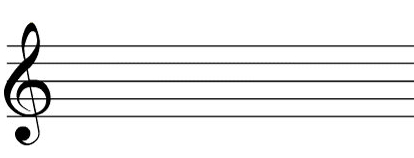
\includegraphics[width=0.8\textwidth]{./imagenes/pentagrama}
  \caption{Representación gráfica de un pentagrama} \label{fig:pentagrama}
  \end{figure}
\item Pulso: es el latido constante y regular de la música, siendo la unidad temporal básica y, en comparación con esta unidad de tiempo, se mide la duración de las notas y silencios.
\item “Tempo”: es la velocidad del pulso. Para indicar un tempo se utiliza como unidad los “bpm” (“Beats Per Minute”, es decir, los “Pulsos Por Minuto”). Así, si el tempo de una obra es de 60 bpm, tendremos que se producirá un pulso por segundo (1 bps) o lo que es lo mismo, cada un segundo, tendremos un pulso.
\item Ritmo: es la combinación de sonidos y silencios de diferente duración.
\item Compás: facilita la lectura de la música. En un pentagrama, los compases quedan divididos por líneas divisorias. Tomaremos que todos los compases son cuaternarios de subdivisión binaria (la mayoría de las obras para banda de música se encuentran compuestas para este tipo de compases o binarios -encajables en los anteriores- y así podremos simplificar el problema para su estudio aunque, como veremos durante la fase de implementación, esto es solo importante para entender mejor el diseño), es decir, un compás está dividido en cuatro notas negras (cada una será de un pulso de duración).
\end{itemize}

\section{Producto a desarrollar}

\paragraph{
Teniendo en cuenta todo lo dicho en las anteriores páginas, es el momento de manifestar qué dispositivo es el que se desea desarrollar en este trabajo: un sistema que marque el pulso (que no el ritmo, al poder ser éste irregular mientras que el pulso es constante) en función del “tempo” que indique el director de la agrupación. Además, el sistema deberá ser discreto ya que se busca que las bandas lo utilicen principalmente en la calle.
}

\paragraph{
Esta necesidad por parte de las bandas de música ha sido detectada por algunos fabricantes, como Peterson, que puso a la venta un producto llamado “Body Beat”. Dispone de un amplio abanico de funciones, pero su tamaño y su elevado coste hacen inviable la implantación del sistema en una banda de música (hay que tener en cuenta que el número de componentes en una banda es variable pero ronda entre los 50 y 100 músicos -algunas de ellas sobrepasan este número, como la “Banda de Cornetas y Tambores Nuestra Señora de la Victoria” conocida como “Las Cigarreras” de Sevilla \cite{cigarreras} que, en las fechas en las que se escribe este trabajo, ronda los 140 componentes-. Por otro lado, las dimensiones, de unos 10.8 cm x 7.6 cm x 2.54 cm puede que sean demasiado grandes). Como último escollo, muchos son los usuarios que, a través de la red, se quejan de la corta duración de la batería (teniendo en cuenta que hay actuaciones que pueden llegar a durar entre 8 y 10 horas, esto es un problema importante).
}

\paragraph{
Un dispositivo más barato con un número menor de funciones pero que permita la sincronización de todos los dispositivos y mantener el tempo durante toda la interpretación, atraería más usuarios. Si además se procura que la construcción se haga utilizando software y hardware libre, podría crearse una comunidad de desarrolladores en torno al producto, consiguiendo mejorar la calidad del dispositivo y aumentar la funcionalidad de este.
}

%
%\input{capitulos/02_EspecificacionRequisitos}
%
%\input{capitulos/03_Planificacion}
%
%\input{capitulos/04_Analisis}
%
%\input{capitulos/05_Diseno}
%
%\input{capitulos/06_Implementacion}
%
%\input{capitulos/07_Pruebas}
%
%\input{capitulos/08_Conclusiones}
%
%%\chapter{Conclusiones y Trabajos Futuros}
%
%
%%\nocite{*}
%\bibliography{bibliografia/bibliografia}\addcontentsline{toc}{chapter}{Bibliografía}
%\bibliographystyle{miunsrturl}
%
%\appendix
%\input{apendices/manual_usuario/manual_usuario}
%%\input{apendices/paper/paper}
%\input{glosario/entradas_glosario}
% \addcontentsline{toc}{chapter}{Glosario}
% \printglossary
\chapter*{}
\thispagestyle{empty}

\end{document}
